A área de tradução automática tem passado por transformações significativas ao longo dos anos, seja pela evolução de modelos específicos por meio de técnicas de otimização, seja pela proposição de novas arquiteturas que estabeleceram novos estados da arte. Este capítulo tem como objetivo apresentar um panorama da evolução das técnicas e modelos de tradução automática, desde as abordagens iniciais até os métodos mais recentes, discutindo suas principais características, vantagens e limitações.

\section{Tradução Automática Baseada em Regras}
A tradução automática baseada em regras, do inglês Rule-Based Machine Translation (RBMT), consiste em sistemas que operam com base em um conjunto de regras linguísticas previamente definidas para a língua de destino. Esses sistemas utilizam regras gramaticais para realizar a tradução entre línguas, exigindo um esforço humano significativo na elaboração de todos os componentes necessários para a tradução de uma língua de origem para uma língua de destino.

Entre esses componentes, destacam-se analisadores morfológicos, etiquetadores de classes gramaticais, analisadores sintáticos, dicionários bilíngues, regras de transferência, geradores morfológicos e regras de reordenação, entre outros \cite{DBLP:journals/corr/abs-1708-04559}.

A Figura \ref{fig:rbmt-processo} ilustra o processo de tradução baseado em regras. Nela, uma frase em inglês é fornecida para o sistema, e baseado nas regras pre-definidas da língua portuguesa como língua de destino a tradução é gerada.

\begin{figure}[H]
	\caption{\label{fig:rbmt-processo}Tradução Automática Baseada em Regras}

	\centering
		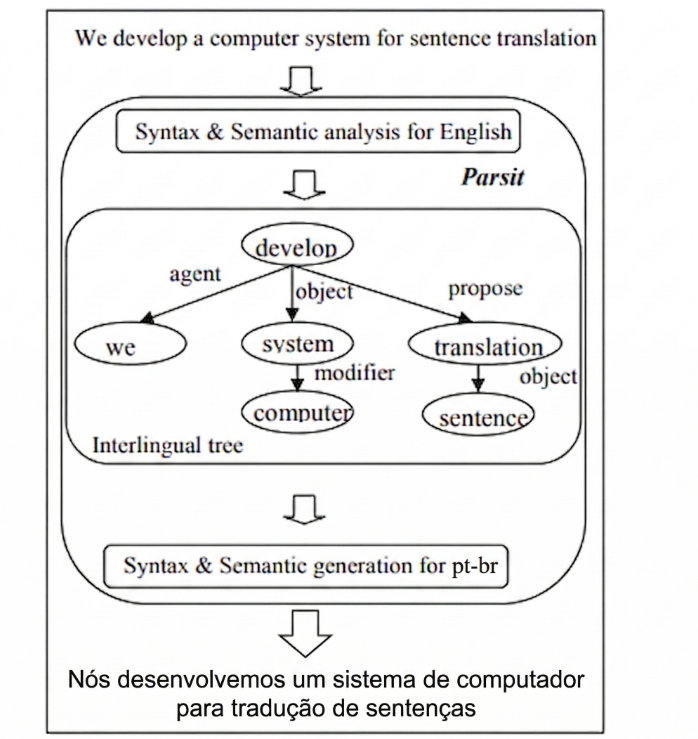
\includegraphics[width=.80\textwidth]{Imagens/RBMT-estado-da-arte.png}

	\legend{Fonte: \cite{charoenpornsawat2002improving} adaptada para português}
\end{figure}

A tradução automática baseada em regras teve início na década de 1970, sendo considerada um marco na área de tradução automática e uma abordagem inicialmente promissora \cite{wiki:Rule-based_machine_translation}. No entanto, algumas características limitaram sua adoção em larga escala \cite{okpor2014machine}:

\begin{itemize}
    \item Escassez de dicionários bilíngues de alta qualidade, sendo sua construção uma tarefa custosa;
    \item Necessidade de configuração manual de diversas informações linguísticas;
    \item Dificuldade em lidar com ambiguidade linguística e expressões idiomáticas, especialmente em sistemas de grande escala.
\end{itemize}

Devido a essas limitações, tornou-se necessária a criação de novas abordagens capazes de lidar melhor com ambiguidade, dependências contextuais entre palavras e reduzir a necessidade de intervenção humana na construção das traduções. Nesse contexto, surgiu a tradução automática baseada em Estatística (Statistical Machine Translation – SMT), que será abordada na na próxima seção.


\section{Tradução Automática Estatística}
A abordagem estatística de tradução baseia-se em modelos probabilísticos extraídos de bases textuais bilíngues alinhadas, nos quais cada palavra ou frase da língua de destino é associada a elementos da língua de origem segundo uma determinada probabilidade. Dessa forma, as palavras ou expressões com maior probabilidade, dentre as opções geradas pelo modelo, tendem a corresponder à tradução mais adequada \cite{DBLP:journals/corr/abs-1708-04559}.

Em termos práticos, um modelo de tradução estatística é treinado com grandes volumes de textos paralelos, contendo a língua de origem e sua tradução correspondente na língua de destino. A partir desses dados, o modelo aprende padrões de correspondência entre palavras e frases, sendo capaz de estimar a tradução mais provável com base nas ocorrências observadas durante o treinamento \cite{lokalise_smt_2025}.

O processo de tradução estatística envolve dois módulos principais: o modelo de tradução e o modelo de linguagem \cite{wang2017neural}.

O modelo de tradução tem como objetivo mapear como palavras ou frases em uma língua geralmente se correspondem em outra, realizando essa análise no nível de frases, e não apenas de palavras isoladas. Esse cuidado evita traduções que não respeitem o contexto, já que uma mesma palavra na língua de origem pode ter múltiplas traduções possíveis na língua de destino.

O modelo de linguagem, por sua vez, recebe os possíveis mapeamentos gerados pelo modelo de tradução e seleciona a frase que apresenta a maior probabilidade de ocorrência na língua de destino, considerando padrões aprendidos a partir dos textos da base de observação. Esse módulo é essencial para produzir traduções mais naturais, que se aproximem do resultado esperado de uma tradução humana.

A imagem abaixo exemplifica este processo de tradução baseado no modelo estatístico. 

\begin{figure}[H]
	\caption{\label{fig:smt-processo}Tradução Automática Baseada em estatística}

	\centering
		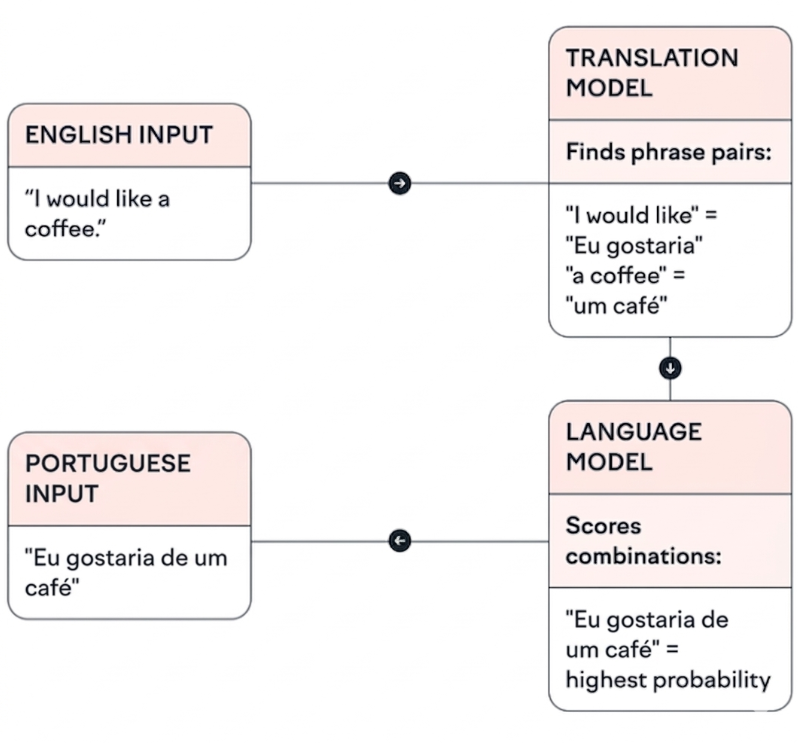
\includegraphics[width=.80\textwidth]{Imagens/estatistica-estado-arte.png}

	\legend{Fonte: \cite{lokalise_smt_2025} adaptada para português}
\end{figure}

É notável que traduções baseadas em estatística superaram traduções baseadas em regras, em qualidade e contexto, porém, os seguintes pontos podem ser destacados sobre traduções estatísticas \cite{wang2017neural}:

\begin{itemize}
    \item Criação de base de dados complexa;
    \item Resultados inesperados. Fluência superficial pode ser enganosa;
    \item Tradução baseada em estatística não funciona bem entre línguas que possuem ordem de palavras diferentes;
    \item Os resultados obtidos tendem a ser mais favoráveis para línguas europeias.
    \item Dificuldade em lidar com dependências de longa distância em frases.
\end{itemize}

Para contornar os problemas listados acima, um novo modelo foi proposto, o qual foi a base para construção de modelos utilizados atualmente, conhecido como aprendizado profundo, em inglês, deep learning, que será abordado no próximo capítulo.

\section{Tradução automática neural}

A tradução automática neural, em sua essência, utiliza redes neurais artificiais (Artificial Neural Networks - ANN), cujo objetivo é simular, de forma simplificada, o funcionamento do cérebro humano. Em termos gerais, o sistema recebe uma entrada, neste caso, um texto na língua de origem, e por meio de módulos internos da rede neural, realiza a tradução para a língua de destino \cite{laratranslate2025neural}.

O processo de tradução é realizado por meio de dois componentes principais: o codificador (encoder) e o decodificador (decoder) \cite{wang2022progress}.

O componente de codificação tem como objetivo mapear o texto de entrada em um vetor de valores reais de múltiplas dimensões. Esse vetor representa, de forma abstrata, informações relevantes necessárias para a realização da tradução. A partir dessa representação vetorial, o componente de decodificação utiliza essas informações para gerar o texto correspondente na língua de destino.

De forma geral, o processo de tradução automática neural pode ser descrito pelas seguintes etapas \cite{laratranslate2025neural}:

\begin{itemize}
    \item Conversão das palavras em vetores numéricos;
    \item Processamento desses vetores por meio de uma rede neural com múltiplas camadas;
    \item Geração de uma distribuição de probabilidade para possíveis traduções;
    \item Seleção da tradução mais provável.
\end{itemize}

A Figura \ref{fig:nmt-processo} ilustra o processo de tradução utilizando redes neurais artificiais, destacando os componentes de codificação e decodificação.

\begin{figure}[H]
	\caption{\label{fig:nmt-processo}Tradução automática neural}
	\centering
	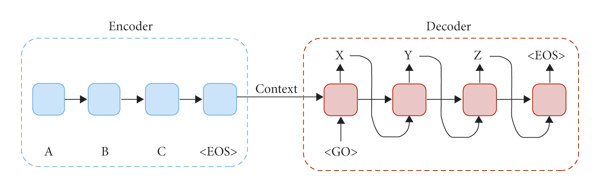
\includegraphics[width=.80\textwidth]{Imagens/encoder-decoder-estado-arte.png}
	\legend{Fonte: \cite{elaffendi2022beyond}}
\end{figure}

O uso da tradução automática neural (Neural Machine Translation – NMT) representou, por muitos anos, uma substituição às técnicas de tradução baseadas em métodos estatísticos. Com a utilização da NMT, tornou-se possível gerar traduções sem a necessidade de intervenção humana direta, baseando-se inteiramente em grandes bases de textos e suas respectivas traduções, abordagem conhecida como aprendizado fim a fim (end-to-end) \cite{laratranslate2025neural}. 

Essa abordagem possibilitou a geração de traduções com maior captura de contexto e maior naturalidade quando comparadas às traduções estatísticas e baseadas em regras, além de melhorar a modelagem das relações entre palavras em uma sentença, um dos principais desafios enfrentados pelas abordagens anteriores \cite{wang2017neural}. 

Um marco importante na adoção da tradução automática neural foi a substituição dos modelos estatísticos pelo uso de NMT no Google Tradutor, realizada pela empresa Google em 2016 \cite{schuster2016zeroshot}, evidenciando uma mudança significativa na forma como sistemas de tradução eram desenvolvidos até então.

Apesar dos avanços proporcionados pela tradução automática neural em relação aos métodos anteriores, ainda existem limitações associadas aos modelos baseados em componentes de codificação e decodificação. Dentre essas limitações, destacam-se \cite{laratranslate2025neural}:

\begin{itemize}
    \item Dificuldade na paralelização do processamento de sequências de entrada;
    \item Limitações no tratamento de dependências de longo alcance entre palavras;
    \item Maior complexidade no processo de treinamento;
    \item Qualidade inferior em determinados cenários de tradução.
\end{itemize}


Com o objetivo de contornar essas limitações, novas abordagens foram propostas, incluindo o uso de mecanismos de atenção, melhorias na paralelização e, posteriormente, o desenvolvimento da arquitetura Transformer.\cite{DBLP:journals/corr/VaswaniSPUJGKP17} 

Dessa forma, o próximo capítulo tem como objetivo apresentar essas abordagens, bem como conceitos relacionados que contribuem para o entendimento da evolução dos modelos de tradução automática neural até os modelos mais recentes, que apresentam elevado desempenho na tarefa de tradução entre línguas.



